\documentclass[12pt]{report}
\usepackage[T1]{fontenc}
\usepackage[utf8]{inputenc}
\usepackage{graphicx}
\usepackage{amsmath,amssymb,amsfonts}
\usepackage{txfonts}
\usepackage{url}
\usepackage{fixltx2e}

% \usepackage{parskip}

%\usepackage[polish]{babel}

\renewcommand{\chaptername}{Chapter}
\renewcommand{\contentsname}{Table of contents}
\renewcommand{\figurename}{Fig.}
\renewcommand{\tablename}{Tab.}
\renewcommand{\listfigurename}{List of figures}
\renewcommand{\listtablename}{List of tables}
\renewcommand{\bibname}{Bibliography}

\renewcommand{\labelitemi}{$\diamond$}

\pagestyle{headings}

\setlength{\textwidth}{14cm}
\setlength{\textheight}{20cm}

% \setlength{\parindent}{20pt}

\newtheorem{definition}{Definition} % przykład nowego środowiska 
\newtheorem{example}{Example}[chapter] % przykład nowego środowiska 
\newtheorem{corollary}{Corollary}[chapter] % przykład nowego środowiska [corollary => wniosek] 



\begin{document}
\tableofcontents	% generuje spis treści ze stronami !!!

%\indent - wymuszony odstep
%\bf - pogrubienie

\chapter{Introduction} \label{rozdz.wstep} 
In the age of ubiquitous Internet access more and more human activities take place in the Web. E-commerce, the act of shopping online, has been on the increase for many years. [{\bf tutaj jakies statystyki, dane nt udzialu ecommerce w ogolnej sprzedazy}]

The amount of products offered on the Internet can be overwhelming for an average consumer, therefore companies take efforts to properly target users with relevant content. Correct product targeting directly translates to increased sales. [{\bf jakis reference}] Systems responsible for this are {\bf recommender systems}.

In the last several years the world has witnessed the rise of social media - Internet-based applications enabling users to connect with each other and share various content. The principal services include Facebook, Twitter and LinkedIn. This phenomenon enabled large-scale user information gathering. That information can be shared with third parties (with user consent) and can be used by them to improve user experience. [{\bf doszlifowac}]

The use of social media in e-commerce is commonly referred to as {\bf social commerce}. According to Lora Cecere of Altimeter Group \cite{rise_of_social_commerce}, "Social Commerce is the use of Social Technologies to connect, listen, understand and engage to improve the shopping experience."

% The aim of this thesis is to create a recommender system that leverages user social media information to suggest products. The implementation will be a demo web e-commerce store.[{\bf rozwinac?}]


% Tutaj ogólnie w skrócie o wzroście znaczenia ecommerce, social commerce etc.
% Coraj więcej produktów, czasem trudno się w tym odnaleźć.
% Rekomendacje dobre zarówno dla klientów (szybciej mogą znaleźć to, czego potrzebują), jak i dla sklepów (większe zyski).

\section{Scope of work}
The thesis involves the areas of software engineering, web development, systems integration and recommender systems.

The aim of this thesis is to design and create a recommender system that leverages users' social media information to suggest products. 

While there exist many recommender systems, most of them require initial information about user preferences regarding some part of data that the later recommended items come from. For example, if a user is to be recommended a movie to watch, the system needs either a history of movies the user has seen, his ratings on multiple movies etc. [{\bf dopracowac}] Next, this information can be processed in two ways:
\begin{itemize}
\item collaborative filtering - based on item ratings, other users with similar tastes are found and items they like are proposed
\item content-based filtering - based on item ratings, items similar to the highest ranked items are found and proposed
\end{itemize}



Są już systemy rekomendacyjne, ale cierpią na 2 główne problemy: cold start i data sparsity. 
Wykorzystanie grafowej bazy danych, dobrze modelującej relacje społeczne.

Osoba podejmująca tematykę stoi przed wyzwaniami: zbudować rzetelną bazę produktów, bazę użytkowników, przekonać użytkowników do udostępnienia danych osobowych etc.

Spodziewane efekty:\\
- rzetelne rekomendacje tuż po zalogowaniu użytkownika\\
- ...\\

% Dlaczego podejmowanie tej tematyki jest potrzebne? Czy są inne
% rozwiązania tego problemu/tych problemów? Jakie? czy są lepsze/gorsze,
% tańsze/droższe, itp.
% \indent Przed jakimi wyzwaniami stoi osoba podejmująca tematykę? \\
% \indent {\bf Określić spodziewane efekty pracy:} W wyniku doświadczeń przeprowadzonych w zakresie pracy polepszeniu
% uległo.... podać konkretne wskaźniki rezultaty, jak np. przyspieszenie obliczeń,
% redukcja kosztu, nowe oprogramowanie itp. w złotówkach, sekundach, procentach,
% roboczogodzinach itp. 

% {\bf (razem max. 3 strony - strona przeliczeniowa = 1800 znaków, średnio 30
% wierszy po 60 znaków)}

\section{Objectives}
% Wymienić w punktach cele pracy, rozpoczynając od celów poznawczych (dotyczą\-cych
% zebrania wiadomości, przybliżenia/popularyzacji technik / metod / zagaadnień).
% W~drugiej kolejności wyienić cele praktyczne.
% \subsubsection{Przybliżenie (popularyzacja) metody/technologii/systemu...}
% \subsubsection{Propozycja rozwiązania problemu....}
% \subsubsection{Opis zastosowania technologii X w problemie Y...}
% \subsubsection{Przedstawienie prototypu systemu/układu/aplikacji...}
% \subsubsection{Określenie przydatności algorytmu Z do rozwiązania problemu T.....
% }
% \subsubsection{Opracowanie strategii ... w celu poprawy wydajności/jakości...}
% \subsubsection{Ocena możliwości wdrożenia proponowanych rozwiązań, ich wartość
% praktyczna, lokalne i globalne możliwości zastosowania}
% \subsubsection{itp.}

% Każdy cel opisać w minimum 2-3 zdaniach. Użyte określenia muszą być powszechnie
% zrozumiałe, nie stosujemy skrótów, slangu,  tzw. makaronizmów, np. ,,softłer''.
% {\bf cały podrozdział ok. 1 strony przeliczeniowej czyli 1800 znaków}

\section{Research method}
% \begin{itemize}
% \item Studia literaturowe
% \item Analiza budowy i działania istniejących produktów
% \item Projektowanie i prototypowanie nowatorskich rozwiązań 
% \item Obliczenia i ........
% \end{itemize}

% Każdy element opisać w minimum 2-3 zdaniach. Np. studia literaturowe powinny
% odnosić się do charakterystyki wykorzystanych źródeł książkowych, czyli: Jaka
% jest podstawowa literatura dziedziny, czy jest dostępna w języku polskim, czy trzeba je tłumaczyć, czy wiedza na ten
% temat jest zebrana w jednym miejscu, czy jej synteza jest osobnym zadaniem itp. 
% Jak duży jest udział źródeł elektronicznych w tej ,,działce'' wiedzy i badań,
% itd. \\
% \indent Jakie metody badawcze są typowe dla danego tematu. Dlaczego je
% zastosowano, ewentualnie dlaczego zastosowano inne? \\
% WYMAGANE ODNOŚNIKI DO POZYCJI BILIOGRAFII.\\
% {\bf cały podrozdział ok. 1 strony przeliczeniowej czyli 1800 znaków}.

\section{Literature overview} % ?? czy to będzie ?
% Rozszerzyć odpowiedni podpunkt z metody badawczej, np. wg podziału:
% \subsubsection{Źródła książkowe polskojęzyczne i tłumaczenia}
% \subsubsection{Źródła książkowe obcojęzyczne}
% \subsubsection{Artykuły naukowe, raporty z badań, komunikaty konferencyjne,
% dokumentacje techniczne, manuale, instrukcje}
% \subsubsection{Źródła elektroniczne}


\section{Thesis plan}
% Tematem pracy jest: ....., zaś za główny cel przyjęto ...... . \\
% Rozdział \label{rozdz.wstep} zawiera wstęp i cele pracy. W rozdziale drugim
% opisano/...... w Rozdziale 3. zawarto............ Rozdział 4. przedstawia..... \\
% W podsumowaniu pracy przedstawiono..........................., z czego wynika,
% że ................  \\
% Najważniejszym wnioskiem/wynikiem/rezultatem pracy jest..................\\ {\bf wyraźnie określić
% CO TO JEST}. \\

% {\bf cały podrozdział ok. 1 strony}.




\chapter[Fundamental information on social...]{Fundamental information on social commerce, recommendation algorithms and graph databases} \label{fundamental_info}

\section{Social Commerce}

- opisać social media?\\
- opisać e-commerce?\\

Social commerce is the fusion of social media with e-commerce \cite{social_commerce_syzygy}. It uses social media, which are founded on user interactions and contributions, to improve the shopping experience on the Internet.

The term itself was created by Yahoo! in 2005, referring to an online place where people can share opinions and experiences, find products and services and buy them. Nevertheless, the roots of such practices date back to 1995, when Amazon started encouraging customers to rate and review products they had purchased.\footnote{\cite{social_commerce_syzygy}, p.4}

In the recent years, however, the popularization of social media services such as Facebook or Twitter has given rise to new social commerce tools and opportunities. Examples include social media stores, i.e. storefronts present directly on the social media sites, or portable social graphs, which give access to users' data to third parties. It is the latter that will be of interest to us in the context of this thesis.

% There are various tools and approaches in social commerce. Examples include social shopping, where we can chat with friends

Social commerce can give businesses the following advantages\footnote{\cite{social_commerce_syzygy}, p.2}:
\begin{itemize}
\item social media monetization
\item e-commerce sales optimization
\item business model innovation
\end{itemize}

From the customer's point of view, the buying experience can be improved in the following ways\footnote{\cite{social_commerce_syzygy}, p.2}:
\begin{itemize}
\item product discovery (social commerce acts as an Awareness Booster)
\item product selection (Decision Accelerator)
\item product referral (Advocacy Activator)
\end{itemize}

According to Dr Paul Marsden of Syzygy Group \cite{social_commerce_syzygy}, there are six dimensions or toolsets for social commerce:
\begin{enumerate}
\item Social Shopping
\item Ratings and Reviews
\item Recommendations and Referrals
\item Forums and Communities
\item Social Media Optimization
\item Social Ads and Apps
\end{enumerate}

In this thesis I will focus only on the Recommendations approach to social commerce.

[TODO]

\section{Recommender Systems}

\subsection{Title?}

Recommender Systems (RSs) are software tools and techniques generating recommendations for items that might be interesting to a user \cite{rec_sys_handbook}. "Item" is a general term referring to what the system can recommend. It can be almost anything, from movies to watch, music to listen to, products to buy, news to read etc.

One category are the non-personalized recommendations. These typically are the "top" lists, such as "top 10 best rated movies", "top 50 most shopped products". They are simple and may provide a good starting point when no information about a user is known, however they are not in the scope of the RS research.

% It is the personalized recommendations that are tackled by RSs.
What the RSs deal with are personalized recommendations. They can be seen as ranked lists of items, most suitable for a user, based on his preferences. To create such a list, the RS requires either explicit user preferences, e.g. ratings of items, or implicit information, i.e. which products the user browsed, how long did they look at each product, what music have they listened to recently.

RSs are based on the observation that people tend to follow recommendations of others while making everyday decisions \footnote{\cite{rec_sys_handbook}, p.2}. Moreover, the second assumption is that if we have similar tastes to someone else, their recommendation would be more accurate than that of a random stranger.

[Functions of recommender systems? (\cite{rec_sys_handbook})]

\subsection{Recommendation Techniques}

In order to be able to suggest items, a RS must implement a way of predicting the utility of an item to the user. Typically this degree of utility of an item \textit{i} for the user \textit{u} is modelled as a function \textit{R(u,i)}. Then the RS has to predict the value of \textit{R} for each user-item pair - compute \textit{\^{R}(u,i)}, where \textit{\^{R}} is the estimation of the true function \textit{R}. Therefore, for each user, having calculated the prediction on a set of items, i.e., \textit{\^{R}(u,i\textsubscript{1}),...,\^{R}(u,i\textsubscript{N})} the system will recommend the items \textit{i\textsubscript{j\textsubscript{1}},...,i\textsubscript{j\textsubscript{K}}} ($K \leq N$) with the largest predicted utility\footnote{\cite{rec_sys_handbook}, p.10}.

The two most popular classes of recommender systems are {\bf content based} and {\bf collaborative filtering} RSs.\footnote{\cite{rec_sys_handbook}, p.11}

% \subsubsection{Content based}
\hbox{}
{\bf Content based:} The recommended items are similar to the ones that the user liked in the past. Similarities between items are calculated on the basis of their features, e.g. in the case of movies it can be their genre, actors, director etc.

The advantage of such an approach is that there is no need for other users in the system. It could work even if only a single user was using it.

However the disadvantage is that all items need to be well characterised by features, which imposes constraints on item addition. Moreover, only items of the same category can be compared, as it is impossible to directly compare features of, e.g. a movie and a music album. Therefore this kind of system could not work well in a multi-category environment.

% \subsubsection{Collaborative filtering}
\hbox{}
{\bf Collaborative filtering:} The idea is to recommend to the active user the items that other users with similar interests liked in the past. The similarity between two users is calculated on the basis of their past ratings of items. Then, if the RS finds that e.g. user B is most similar to the active user A, it will find items highly rated by B that A has not yet rated (thus probably does not know) and recommend them to user A.

This approach to RS allows for the items to be transparent to the system, i.e. it does not need to know what the items are nor what features, properties they have (as opposed to the content-based approach). It allows for greater flexibility when it comes to adding items.

The drawback is that in order for the system to work, it needs a large user base with ratings. Moreover, if a new item is added in the course of the system's functioning, it will be available for recommendations only after some users have rated it.

\hbox{}
There exist other types of recommender systems...

[TODO: opisać tutaj community-based (\cite{rec_sys_handbook}, p.13) jako podobny do mojego, ale bazujący tylko na znajomościach pobranych z SN, a nie na profilach użytkowników]

\subsection{Application}
[TODO: \cite{rec_sys_handbook}, p.14]

\section{Graph databases}

\subsection{Graphs}

A graph is a collection of vertices and edges, or, more simply put, a set of \textit{nodes} and the \textit{relationships} between them \cite{graph_databases}. It is a general purpose structure, where nodes represent entities and relationships - the ways these entities relate to each other.

Graph theory, the study of graph models and algorithms, has been used in many disciplines \cite{learning_neo4j}:
\begin{itemize}
\item {\bf Social studies}: Human beings are a social species, we are interconnected by relations. People interact with people every day, exchange items, ideas, therefore modelling those interactions with graphs seems natural.
\item {\bf Biological studies}: Biological components and their interactions can be modeled as a graph structure, which has many practical advantages.
\item {\bf Computer science}: The usage ranges from chip design, network management, recommendation systems, UML modeling to algorithm generation and dependency analysis.
\item {\bf Flow problems}: Used in telecom / gas / airline / package delivery networks to find the optimal path, bottlenecks, for capacity planning etc. 
\item {\bf Route problems}: To find the optimal route between two nodes on a network, e.g. car navigation systems.
\item {\bf Web search}: The original Google search algorithm, PageRank, was a graph algorithm.
\end{itemize}

[TODO więcej?]

\subsection{Graph Database Management Systems}

The main types of database management systems are:
\begin{itemize}
\item {\bf Relational databases}: Data is organized in tables of rows and columns. Because each row has a unique key, rows in a table can be linked to rows in other tables.
\item {\bf NoSQL databases}: The acronym standing for "Not Only SQL" represents a new generation of databases \cite{learning_neo4j}. These include:
\begin{itemize}
\item Key-Value stores
\item Column-Family stores
\item Document stores
\item Graph databases
\end{itemize}
\end{itemize}

A graph database management system is an online database management system with Create, Read, Update and Delete (CRUD) methods that expose a graph data model \cite{graph_databases}. Graph databases support transactions and are optimized in terms of transactional performance, integrity and operational availability.

When analyzing graph database technologies, it is important to consider the two factors \cite{graph_databases}:
\begin{itemize}
% \item {\bf Underlying storage}: 
% \item {\bf Processing engine}:
\item Underlying storage: Some graph databases use the so-called \textit{native graph storage}, designed solely for storing and managing graphs. Others, however, keep the data in other data stores, e.g. in a serialized form in a relational database.
\item Processing engine: The best performance is gained when a graph database implements \textit{native graph processing}, therefore the connected nodes physically point to each other in the database without the use of indices.
\end{itemize}

\begin{figure}[!t]
\centering
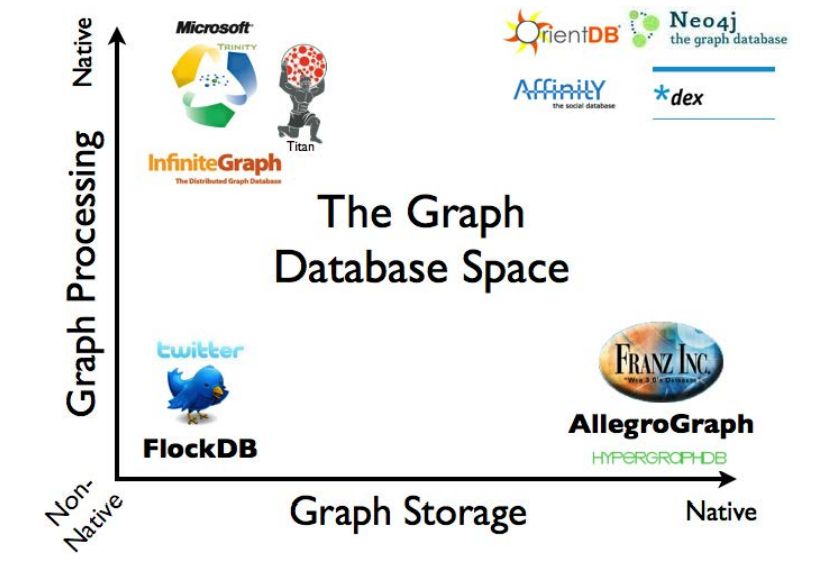
\includegraphics[width=\textwidth]{graph_databases_comp.jpg} 
\caption[Overview of graph databases.]{Overview of graph databases.\footnotemark{}}
\label{fig.graph_databases}
\end{figure}
\footnotetext{Image source: \cite{graph_databases}, p.7}

Figure \ref{fig.graph_databases} presents different graph database implementations in terms of their compliance with the nativity of both graph processing and graph storage. As it can be seen, Neo4j is one of the most advanced implementations in both aspects. Moreover it is very popular and well documented, therefore it was chosen as the graph database engine for this thesis.


\subsection{The Property Graph model}

Data is stored in a graph database using the Property Graph data model \cite{learning_neo4j}. In this model both nodes and relationships can have their \textit{properties}, represented by key--value pairs. It can be characterised by the following:
\begin{itemize}
\item There is no fixed schema.
\item The database can deal with semi-structured data, e.g. some nodes / relationships can have more or less properties than others and it causes no problems.
\item Nodes and their properties are analogous to rows in a table with fields.
\item Relationships are explicit, rather than established with a join operation at runtime. They can also have properties, which is unique as compared to relational databases.
\end{itemize}

Moreover, this data model was customized in Neo4j to allow for two additional important concepts:
\begin{itemize}
\item {\bf Node labels}: Each node can have one or more labels, which are a sort of a "special property". It helps create a type structure. They are useful for creating subgraphs in the database or to fetch only nodes of a specific type.
\item {\bf Relationship types}: Similar to node labels, but for relationships, however they are mandatory. Moreover each relationship can only have one type. They are useful for graph traversals limited to certain kinds of paths only.
\end{itemize}

\begin{figure}[!t]
\centering
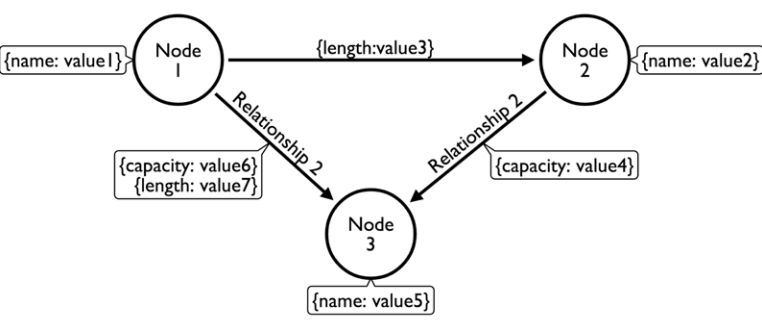
\includegraphics[width=\textwidth]{property_graph2.jpg} 
\caption[Property graph example.]{Property graph example.\footnotemark{}}
\label{fig.graph_databases}
\end{figure}
\footnotetext{Image source: \cite{learning_neo4j}, p.35}

\subsection{Comparison with relational and other NoSQL databases}

Why use a graph database? \cite{learning_neo4j}, p.37

[TODO Join bomb \cite{learning_neo4j}, p.27]

["graph databases actually take relational databases...", \cite{learning_neo4j}, p.33]

[TODO The power of graph databases \cite{graph_databases}, p. 8]

\subsubsection{Performance}

\subsubsection{Flexibility}

\subsubsection{Agility}

\chapter{Presentation of existing recommender systems}

\section{A Social Network-Based Recommender System (SNRS)}


% % %
\chapter{Implementation of new functionalities}

\section{Overview}
\subsection{General idea}
In order to implement and test the system I have decided to build a web application. It is a sample e-commerce store that will gather information about users from their social network. Additionally it will contain a list of exemplary products from different categories, which will be recommendable items. 

The general idea was to implement the so-called "social login" - \cite{social_login} a feature enabling the user to log in to a third-party website using existing login information from a social networking service, without the need of creating a new login account specifically for that website. A website using this feature can request additional information from the user's profile, such as gender, location, list of friends, interests etc. 

Thanks to this, a newly logged user would not be anonymous for my application. By requesting appropriate information from the social network I would be able to analyze user's data and compare them to other existing users in my database. As a result, it would be possible to calculate similarities between users, which is a crucial step in recommender systems.

It is worth noting that the user similarity computation would occur before any interaction of the user with my application. This is a major difference as opposed to classical collaborative filtering approaches, where in order to find nearest neighbours (most similar users) users are compared in terms of their preferences towards recommendable items (e.g. ratings of movies). In my case only the information derived from social networks influences the similarity.

As a consequence, the new approach enables serving recommendations to new users right after their login to the website. The only limiting factor is data downloading from the social network and computation time. Nevertheless, it is safe to assume that the result could be presented withing tens of seconds after the login step. Even if it is not instantaneous, in a typical use case the time needed for recommendation computation would allow the user to get familiar with the website's layout, functionalities etc. When the results would be ready, they could be asynchronously loaded onto the page. 

The only prerequisite for such a situation is that there exists a reasonable user base of the service. Moreover, the system needs to both possess the users' social network information and to know their preferences towards the system's items. Therefore, in a typical scenario of implementation in an existing service, first the social login and social information acquisition would be enabled. After a period of gathering the preferences of socially-logged users, via their item ratings, shopping/browsing history, comment analysis etc., the initial user base would be established. In the second phase, each new user could obtain recommendations. Obviously, the system will improve over time, as more and more users with social data and product preferences are in the database.

\subsection{Solution plan \textit{[?]}}

The system implementation will be conducted in two stages.
\begin{enumerate}
\item Users will be able to log in to the website with their social network account. Next, they will be asked to complete a survey, in which they will rate products in the store's catalog according to their tastes. No recommendation will be offered at this point.
\item Having the initial user base, any new user logging in with the social network will be presented with instant recommendations on products.
\end{enumerate}

The social network that the application will integrate with is Facebook. After research it was found that Facebook can provide most useful user information. Moreover, it is the most popular social network in Poland, therefore it will be easiest to find volunteers eager to provide their data to the project.

\subsection{Technologies}
\subsubsection{Web application}
The main development language is Java 8. The web application is created using Spring Framework 4 \cite{spring_framework}, with Spring MVC as the model-view-controller design pattern implementation and Thymeleaf as the template engine. 

The front-end of the website uses the typical web technology stack: HTML / CSS / JavaScript (jQuery). A free theme for the Bootstrap front-end framework, Lumen \cite{lumen}, was used.

The connection with Facebook was realized with the help of RestFB - a simple Facebook Graph API written in Java \cite{restfb}.

\subsubsection{Database}

Because of the specificity of social relations, i.e. many connections between entities, classical relational databases are not the best choice for modelling such data. Therefore, in order to ensure good performance and scalability, a graph database Neo4j \cite{neo4j} was chosen for data storage.

\subsubsection{Server}

The application is hosted online at the URL: \url{http://store.przedwojski.com/}. 

The hosting provider is Amazon Web Services (AWS). The Spring application runs on a Tomcat server along with an embedded Neo4j database. They are located on an Amazon Elastic Cloud Computing (EC2) micro instance running Linux AMI (Amazon Machine Image), a modified version of CentOS.

The Amazon Route 53, a DNS and Domain Name Registration service, was used to link the domain name to the EC2 instance's IP address.

\section{Web application and social login}
\subsection{Design [ew. inna nazwa]}

The web application consists of 3 main parts:
\begin{itemize}
\item the login screen
\item the survey - used in the first stage to gather user ratings for products
\item the recommender - used in the second stage to provide recommendations
\end{itemize}

\subsubsection{The login}
[{\bf schemat login flow?}]

Upon entering the website, the user is presented with the login screen, shown in Figure \ref{fig.login}. The top panel contains two buttons: "About", which opens up a popup with additional information on the project, and "Report problem", which leads to a form created in Google Forms for submitting any issues with the application.

The central panel contains the login button for Facebook. When clicked, it uses the Facebook Javascript API to open a new window and guide the user through the Facebook authentication process. The user needs to authorize the Facebook application to access their data, as depicted in Figure \ref{fig.login.fb_app_auth}. Once that is completed, the window is closed and a callback to the original page is activated, informing about a successful login.

Depending on the stage of the project, the user is then redirected either to the survey or to the recommendation page. 

\begin{figure}[!t]
\centering
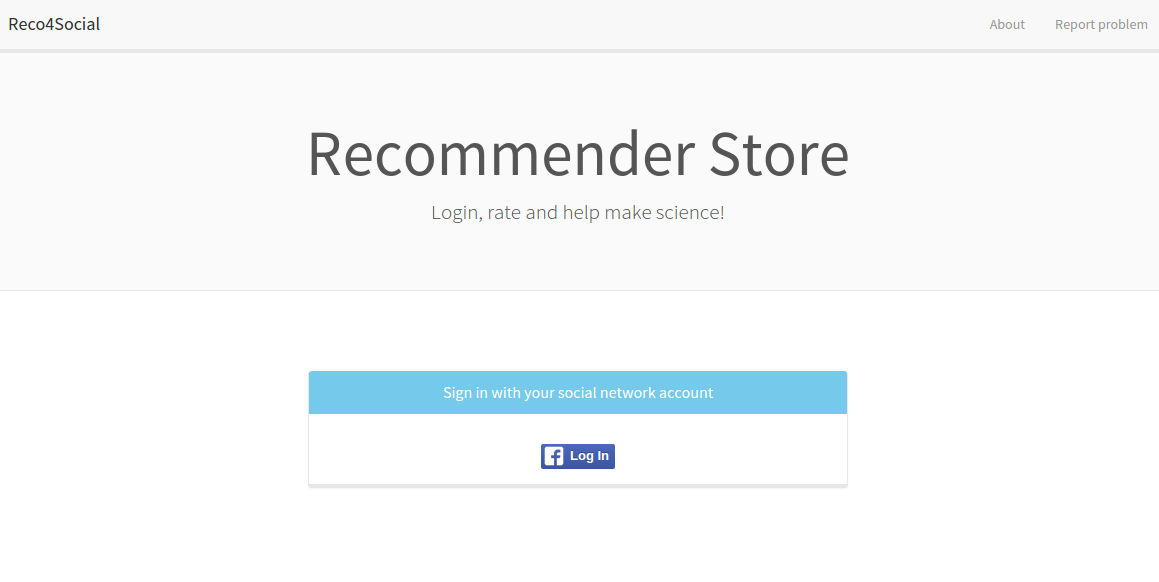
\includegraphics[width=\textwidth]{reco4_login.png} 
\caption[Login page.]{Login page.}
\label{fig.login}
\end{figure}

\begin{figure}[!t]
\centering

\includegraphics[width=7cm]{todo.jpg} 
% width=\textwidth
\caption[Authorizing the Facebook application.]{Authorizing the Facebook application.}
\label{fig.login.fb_app_auth}
\end{figure}

In the background, a Spring component uses the user credentials to query Facebook for additional data. The requested data includes:
\begin{itemize}
\item gender
\item hometown
\item current city
\item political view
\item religion
\item likes - the Facebook pages that the user "likes"
\item friends - only those who have also logged in to my website
\end{itemize}

If during the application authorization process the user edited the sharing options, some or all of the above data may not be accessible.

The received information is processed in the background and stored in the graph database.

\subsubsection{The survey}
\begin{figure}[!t]
\centering
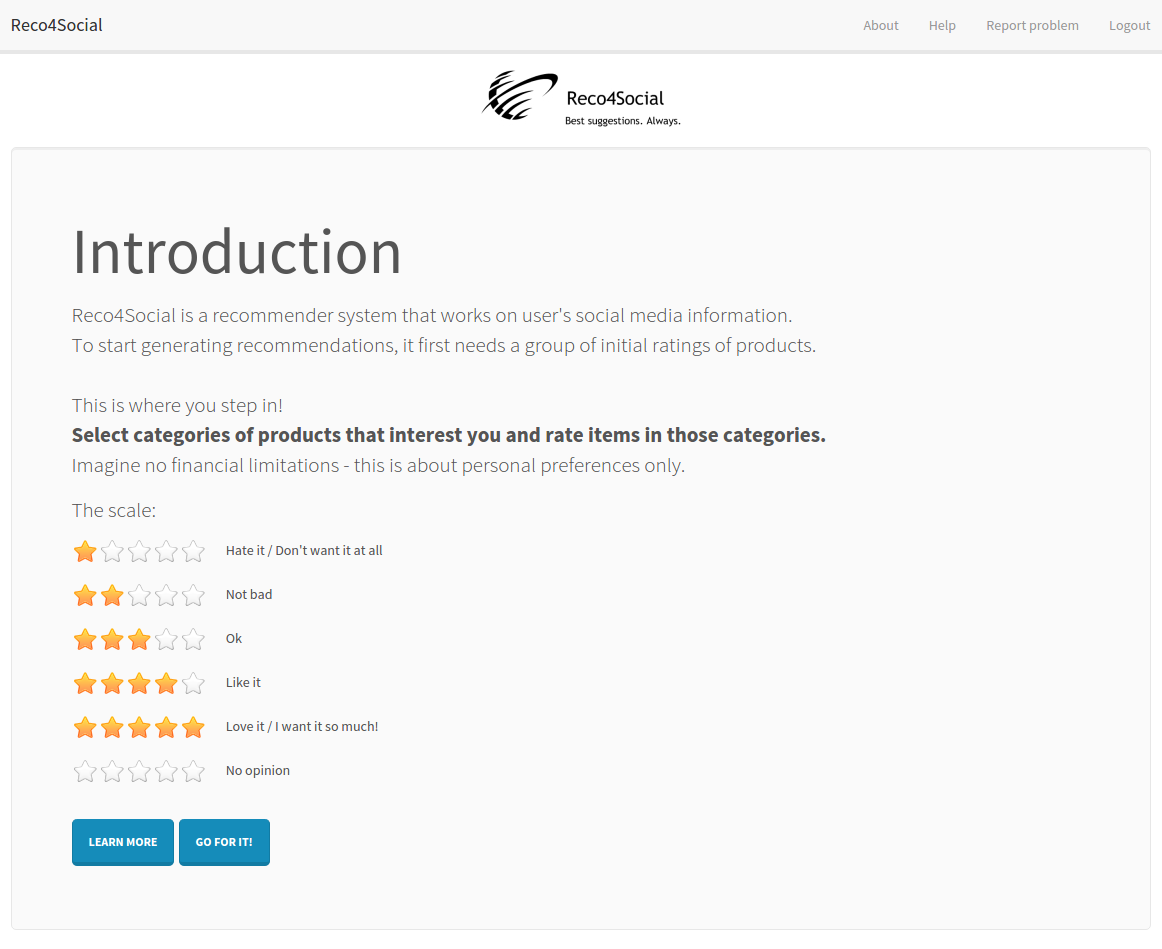
\includegraphics[width=\textwidth]{reco4_survey-intro-1.png} 
\caption[Survey introduction.]{Survey introduction.}
\label{fig.survey.intro-1}
\end{figure}

\begin{figure}[!t]
\centering
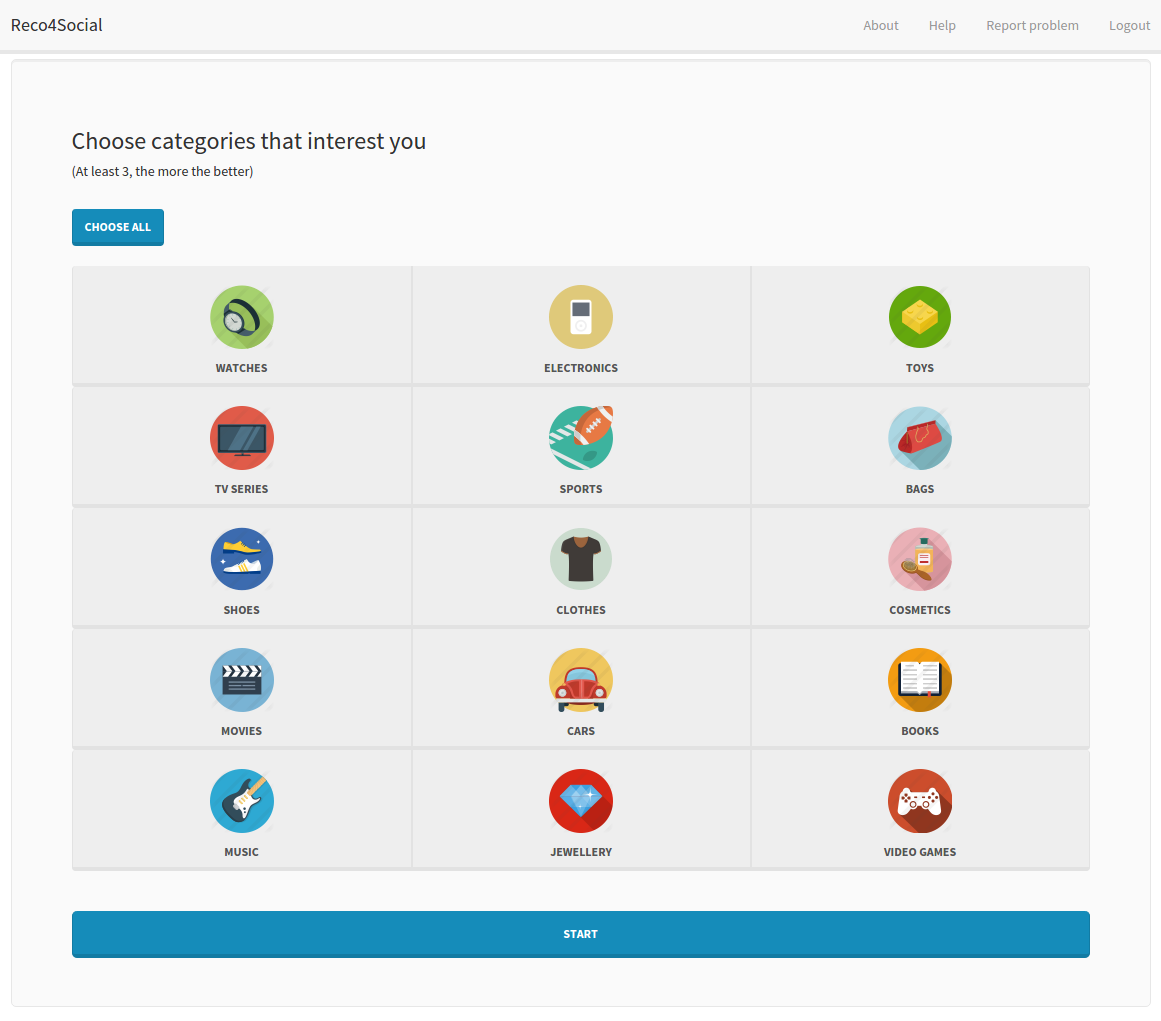
\includegraphics[width=\textwidth]{reco4_survey-intro-2.png} 
\caption[Survey product categories selection.]{Survey product categories selection.}
\label{fig.survey.intro-2}
\end{figure}

\begin{figure}[!t]
\centering

\includegraphics[width=7cm]{todo.jpg} 
% width=\textwidth
\caption[The survey.]{The survey.}
\label{fig.survey}
\end{figure}

\begin{figure}[!t]
\centering

\includegraphics[width=7cm]{todo.jpg} 
% width=\textwidth
\caption[The survey end.]{The survey end.}
\label{fig.survey.end}
\end{figure}

After having successfully logged in, the user is presented with an introduction to the survey, visible in Figure \ref{fig.survey.intro-1}. It explains what the project is about and how to complete the survey, including the description of the rating system.

Users are supposed to choose categories of products that interest them (at least three) and then to rate products in those categories according to their tastes. The rating scale is 1-5, where 1 means "do not like at all" and 5 means "love it". If a user has no opinion about a particular product, they are supposed to leave the rating empty.

For those users that seek additional information about the project, there is the "Learn more" button, which opens a popup window with a more detailed explanation.

Figure \ref{fig.survey.intro-2} shows the categories selection panel, which is located just below the introduction. The users are asked to choose at least three categories, otherwise they are not permitted to proceed. The "Start" button redirects the user to the actual survey.

The survey page (Figure \ref{fig.survey}) presents all products from each category, one at a time. At the top a progress bar informs the user how many categories are left. Each product is contained within a "box", displaying the item's name, picture, price and the rating to be filled. The rating is presented in the form of "stars".

A button at the bottom reloads the page presenting products from the next category. In the case of the last category, it redirects to the survey end page. It is shown in Figure \ref{fig.survey.end} and contains the acknowledgement of the user's contribution to the project.

\subsubsection{The recommender}
[TODO]

\subsection{Implementation}

\subsubsection{Facebook application configuration}
The first step in using the Facebook API is application creation. User data can only be accessed when they grant the appropriate privileges to our application.

The place for managing Facebook applications is the Developer center, available at the URL: \url{https://developers.facebook.com/}.

To properly configure a new App, multiple details need to be provided, including the name, category, type (iOS, Android, web), its domain, website etc. Afterwards, two parameters are generated: App ID and App Secret, that allow client authorization.

When new App is created, at first it possesses only the basic permissions for accessing users' data, namely the \url{public_profile}, \url{email} and \url{user_friends} items.

In order to gain permissions for additional information, an approval submission needs to be filled in. Facebook expects detailed explanation, along with screenshots of the website, of how the obtained data will be used. At first my submission was rejected, however the second time, after having underlined that my project is not commercial, but purely academic, the permissions were granted.

In the end the Facebook App has the following permissions that are used in the project:
\begin{itemize}
\item \url{public_profile}
\item \url{user_friends}
\item \url{user_hometown}
\item \url{user_location}
\item \url{user_religion_politics}
\item \url{user_likes}
\end{itemize}

\subsubsection{The login}

The web application is created with the MVC design pattern in mind. Therefore a \textit{Model} manages the data and logic of the application, a \textit{View} presents data to the user in the form of HTML documents and a \textit{Controller} acts as an intermediary between the two, sending data from a model to a view to display it to the user as well as gathering user input from the view and transmitting the information to the model.



\subsubsection{The survey}

\subsubsection{The recommender}

%
\section{User data model in Neo4j}

\subsection{Introduction to Graph Databases}

\subsection{Data model}

\section{Recommendation algorithm}

\chapter{Evaluation}
\section{Evaluation of predictive and classification accuracy}
\section{Evaluation of computation time and resource consumption}
\section{Comparison to non-social recommender systems}

\chapter{Summary and conclusions}
\section{Usability of the project in AMG.net/Atos}
\section{Future development perspectives}

% \chapter{Bibliography}

% \chapter{Appendices}

\addcontentsline{toc}{chapter}{Bibliography} 
\begin{thebibliography}{99}

\bibitem{rise_of_social_commerce}
Lora Cecere, \textit{Rise of Social Commerce}, Altimeter Group conference presentation, 2010, Available at: \url{http://www.riseofsocialcommerce.com/wp-content/uploads/2010/10/Lora_Cecere-Rise_of_Social_Commerce.pdf}, [access: 1 May 2015].

\bibitem{snrs}
Jianming He, Wesley W. Chu, \textit{A Social Network-Based Recommender System (SNRS)}, Computer Science Department, University of California, Available at: \url{http://www.cobase.cs.ucla.edu/tech-docs/jmhek/snrs.pdf}, [access: 25 April 2015].

\bibitem{social_login}
Loren McDonald, \textit{Social Login: A Data Capture Game Changer}, Silverpop blog (An IBM Company), 29 November 2011, Available at: \url{http://www.silverpop.com/blogs/email-marketing/social-login-data-capture.html}, [access: 28 August 2015].

\bibitem{spring_framework}
Web page of the \textit{Spring Framework}, Pivotal Software, Available at: \url{http://projects.spring.io/spring-framework/}, [access: 28 August 2015].

\bibitem{lumen}
Web page of a Bootstrap theme, \textit{Lumen}, Available at: \url{https://bootswatch.com/lumen/}, [access: 28 August 2015].

\bibitem{restfb}
Web page of \textit{RestFB}, Available at: \url{http://restfb.com/}, [access: 28 August 2015].

\bibitem{neo4j}
Web page of \textit{Neo4j}, Available at: \url{http://neo4j.com/}, [access: 28 August 2015].

\bibitem{social_commerce_syzygy}
Paul Marsden, \textit{Social Commerce: Monetizing Social Media}, Syzygy Group, 2010, pp. 2-12, Available at: \url{http://digitalintelligencetoday.com/downloads/White_Paper_Social_Commerce_EN.pdf}, [access: 1 September 2015].

\bibitem{rec_sys_handbook}
Francesco Ricci, Lior Rokach and Bracha Shapira, \textit{Introduction to Recommender Systems Handbook}, Recommender Systems Handbook, Springer, 2011, pp. 1-35, Available at: \url{http://www.inf.unibz.it/~ricci/papers/intro-rec-sys-handbook.pdf}, [access: 2 September 2015].

\bibitem{graph_databases}
Ian Robinson, Jim Webber and Emil Eifrem, \textit{Graph Databases}, O'Reilly, 2013, pp. VII-IX, 1-... [TODO]

\bibitem{learning_neo4j}
Rik Van Bruggen, \textit{Learning Neo4j}, Packt Publishing, 2014, Available at: \url{http://neo4j.com/book-learning-neo4j/}, [access: 26 March 2015].

\end{thebibliography}

\addcontentsline{toc}{chapter}{List of figures} 
\listoffigures

\addcontentsline{toc}{chapter}{List of tables} 
\listoftables

\end{document}
